\chapter{Laden von Resource-Sets}
\label{resource_sets}

Grundsätzlich muss ein Modell nicht in sich geschlossen sein. Es können auch andere Modelle
importiert werden und Objekte aus diesen Modellen referenziert werden. Bei Ecore basierten Modellen
wird z.B. häufig die Ecore eigene Typbibliothek eingebunden. Diese Typbibliothek stellt primitive
Datentypen zur Verfügung, die z.B. häufig als Attributtyp verwendet werden. Als allgemeine Typen
werden aber zum Teil auch \texttt{EClass}, \texttt{EReference}, \texttt{EAttribute} usw.
verwendet (siehe z.B. Differenzmodell \ref{fig:diffmodel} oder Henshin-Modell
\ref{fig:henshin_metamodel}). Alle importierten Modelle müssen für ein korrektes Semantic-Lifting
ebenfalls Teil der Differenz sein, da deren Modell-Elemente häufig zum Kontext der Editierregel
gehören. Zum Beispiel beim Anlegen eines Attributs, wie in Abbildung \ref{fig:add_eattribute_rule}
dargestellt.

\begin{figure}[htb]
  \centering 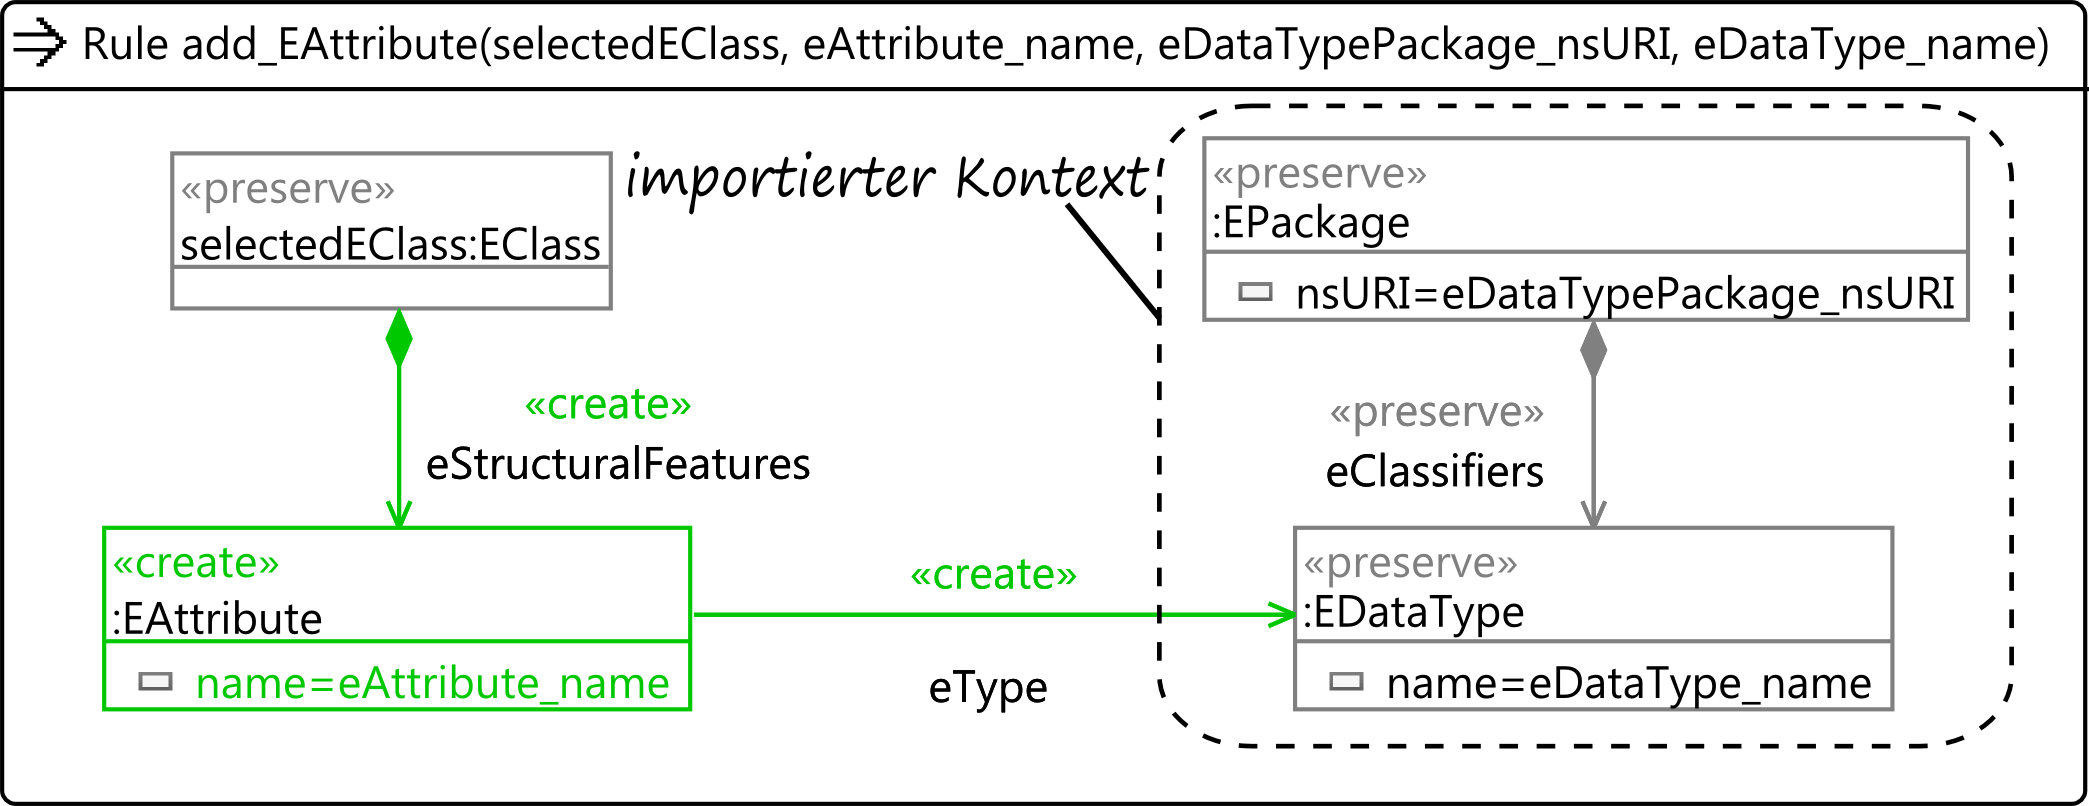
\includegraphics[width=1.0\textwidth]{images/add_eattribute.png}
  \caption{Add EAttribute}
  \label{fig:add_eattribute_rule}
\end{figure}

Aus technischer Sicht können die Modelle auf zwei Arten importiert werden:
\begin{enumerate}
  \item Das importierte Modell, das von Modell A und B referenziert wird, ist das selbe Modell. Dies
  ist in der Regel dann der Fall, wenn das Modell aus der Ecore \textit{package
  registry}\footnote{siehe \cite{SBPM2009} Abschnitt 14.1.2} geladen wurde. Beziehungsweise aus Sicht einer
  Versionsverwaltung hat sich das importierte Modell von Modell A zu Modell B nicht verändert.
  
  \item Im Gegensatz dazu könnte es natürlich auch sein, dass sich das importierte Modell
  ebenfalls verändert hat. D.h. Modell A referenziert eine andere Version dieses Modells als
  Modell B.
\end{enumerate}
Der implementierte Algorithmus befasst sich zunächst nur mit Fällen der ersten Kategorie.
Hauptsächlich mit dem Ziel das Ecore-Metamodell inklusive der Typbibliothek in die Differenz
einzubinden. Der folgende Algorithmus kann aber auch mit allen anderen importierten Modellen der ersten
Kategorie umgehen. Hierzu wird die Differenz nach der Differenz-Ableitung um die importierten
Modelle erweitert. Dabei muss bedacht werden, dass in der Erkennungsregel für jeden importierten Kontext
Knoten nach einer Korrespondenz mit einem passenden Modell A und B Objekt gesucht wird. Da die
Erkennungsregeln injektiv auf die Differenz abgebildet werden, heißt das auch, dass Modell A und
Modell B Knoten nicht auf das selbe Objekt abgebildet werden können. Da aber bei importierten Modellen
der ersten Kategorie nur eine Instanz der Modelle existiert, muss eine Kopie dieser Modelle
erzeugt werden, welche dann in die Differenz eingebunden werden kann. Dazu werden folgende Schritte
ausgeführt:

\begin{enumerate}
  \item Finde alle Referenzen auf importierte Modelle in Modell A und B.
 
  \item Erstelle eine Kopie aller referenzierten importierten Modelle. Bis hierher referenzieren die
  beide Modelle A und B noch die selben Instanzen der importierten Modelle. Als nächstes wird die
  Differenz so umgebaut, dass Modell A die originalen importierten Modelle referenziert und Modell B
  die Kopien.
  
  \item Um die importierten Modelle in die Differenz einzubinden, erzeuge für jedes importierte Modell
  Korrespondenzen (\texttt{Correspondence}) zwischen allen originalen Modell-Element und denen der Kopie.
 
  Um die Differenz durch die importierten Modelle nicht unnötig groß zu machen, gibt es die
  Möglichkeit einen Filter zu implementieren, der festlegt, welche importierten Elemente in die
  Differenz übernommen werden sollen. Der im Rahmen dieses Projekts implementierte Filter übernimmt
  nur die referenzierten importierten Elemente und deren Container in die Differenz. Dies sollte in
  der Regel für Ecore Modelle ausreichend sein.
 
  \item Setze alle Referenzen in Modell B vom Original auf die Kopie des importierten Modells.
  
  \item Setze alle Referenzen von Add-Reference low-level Änderungen vom Original auf die Kopie des
  importierten Modells.
  
  \item Speichert alle Änderungen an der Differenz und an Modell B, damit diese nach dem
  eigentlichen Semantic-Lifting, zum Speichern der Differenz wieder rückgängig gemacht werden
  können.
\end{enumerate}
Der Vorteil des beschriebenen Algorithmus besteht darin, dass kein Matching für die importierten Modelle
berechnet werden muss. Da man die Korrespondenzen der importierten Modelle vom Original zur Kopie 
ohnehin beim Kopiervorgang gleich mit abspeichern kann.

Für importierte Modelle der zweite Kategorie müsste das Matching und die Differenz-Ableitung auf das
gesamte Resource-Set beider Modelle ausgeweitet werden. Vorausgesetzt man verfügt über die
entsprechenden Versionen der importierten Modelle, muss des Weiteren die Laderoutine der Modelle
entsprechend angepasst werden. Es muss z.B. sichergestellt werden, dass die jeweiligen importierten
Modell Versionen auch verwendet werden und nicht eine andere Version aus der Ecore \textit{package
registry} geladen wird. Theoretisch lässt sich dieser Ansatz auch auf Fälle der ersten Kategorie
übertragen. Allerdings nur dann, wenn man Einfluss auf die Laderoutine hat, damit zwei Instanzen
des selben importierten Modells (je für Modell A und B) geladen werden können.